%%%%%%%%%%%%%%%%%%%%%%%%%%%%%%%%%%%%%%%%%%%%%%%%%%%%%%%%%%%%%%%%%%%%%%%%%%%%%%%%%%%%%%%%%%%%%%%%%%%%%%
%
%   Filename    : chapter_3.tex 
%
%   Description : This file will contain your Research Methodology.
%                 
%%%%%%%%%%%%%%%%%%%%%%%%%%%%%%%%%%%%%%%%%%%%%%%%%%%%%%%%%%%%%%%%%%%%%%%%%%%%%%%%%%%%%%%%%%%%%%%%%%%%%%

\chapter{Research Overview}
This chapter contains procedures that propoenents will follow for the research based from theories and concepts discuess in chapter 3 and the methodologies discussed in chapter 1.

\section{System Architecture}

\begin{figure}[h]
\centering
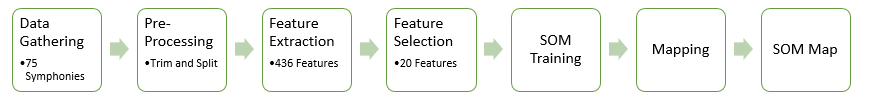
\includegraphics[scale=0.7]{sysarch1}
\end{figure}

\begin{figure}[h]
\centering
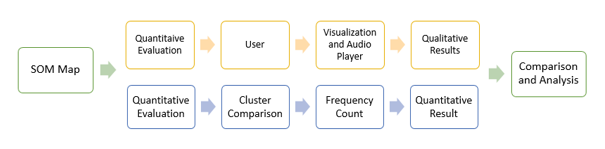
\includegraphics{sysarch2}
\end{figure}

\section{Preprocessing}

After acquiring the symphonies from online sources or through physical means, omitting segments of the music file which has no sound in it will be done using Audacity. This is done so that the output produced later will have no empty values since no sound will result in empty values. After the music files are cleaned, they will then be cut into one second music segments with a half second overlapping interval just as discussed in section 1.5.3 using Direct WAV MP3 Splitter. The music segments will then have their features be extracted using jAudio, producing an output file of XML. The XML file will then be converted to CSV format. The consolidated CSV file of all symphonies will then be used for feature selection to select only the more important features just as discussed in section 3.2.4. After the features have been selected, audio feature extraction will be done again, but only for these selected features. The resulting CSV file will then be used for machine learning using RapidMiner to be used in producing the SOM.

\section{Visualization Components}
\subsection{Function}

The program will allow the proponents to visualize the SOM in 3D by plotting the BMU of each music segment on a 2D plane and then collating the results of all segments in the composition in time series. The result is a line T(x, y, z) where (x, y) denotes the coordinates of the BMU of a particular music segment on the SOM and z being the index of the segment in the time series.

\subsection{Screenflow}

\begin{figure}[h]
\caption{Figure 4.1)}
\centering
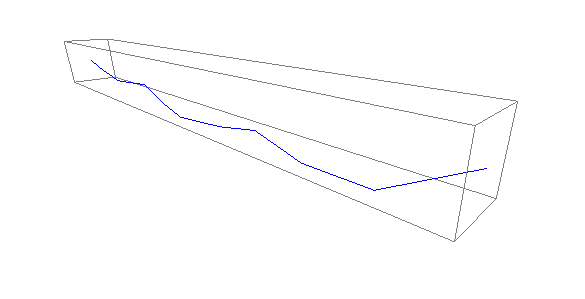
\includegraphics{visual1}
\end{figure}

Displaying the data of one symphony will plot a line that represents the musical trajectory or progression of the symphony in the SOM from start to finish. Each point on the z-axis (longest axis) represents the position of the BMU on the SOM at a particular interval in the time series as shown in Figure 4.1.

\begin{figure}[h]
\caption{Figure 4.2)}
\centering
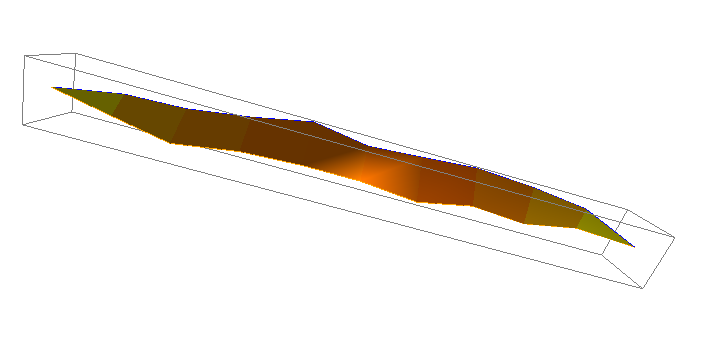
\includegraphics{visual2}
\end{figure}

Alternatively, when comparing two symphonies, two lines will be generated representing the musical trajectories of both symphonies. As shown in Figure 4.2, the area between the two lines will be colored depending on the Euclidean distance between the two BMUs in the same time axis.

\section{Testing and Methodology}
\subsection{Quantitative}

K-means clustering algorithm will be used as the algorithm for machine learning and Euclidean distance will be used for calculating the BMUs for each cluster to compare the similarities of symphonies just as discussed in section 3.5.1.

\subsection{Qualitative}

A survey form deployed online will be used to validate the result for the quantitative measurements. In the survey, the participant will first be asked for their voluntary consent. Then, upon consenting, they will be asked to listen to two symphonies that are found to be similar using the quantitative measure used in the research as seen in figure 4.3. The system will provide suggested time slices for them to annotate. An annotation module is provided for the user to rate the similarity from 1 to 5, with 1 being dissimilar and 5 as similar. They may also choose to annotate which part/parts in the symphony that was not suggested yet they believe were similar. Upon selecting time slices, the coloration of the time slices would change depending on the \% similarity of the selected slice. A spectrum of red to green would be used, with red representing a low \% similarity and green representing a high \% similarity. The results from these should help validate if this research work’s methodology and speculated results prove true.

\begin{figure}[h]
\caption{Figure 4.3)}
\centering
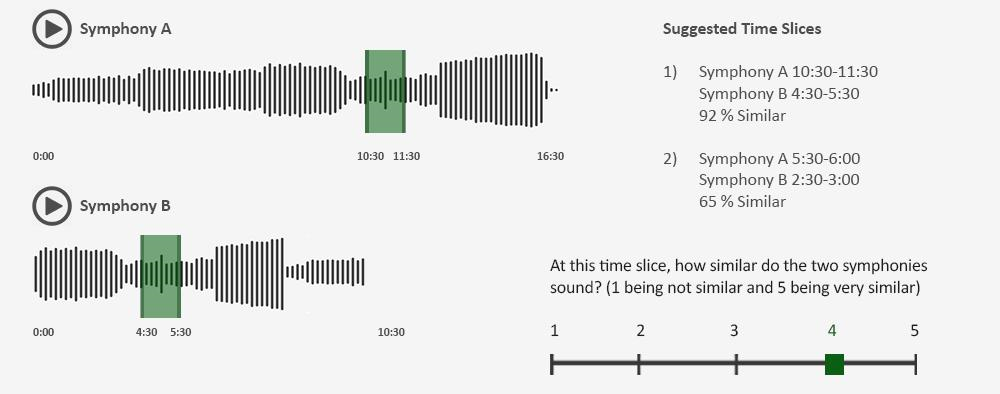
\includegraphics[scale=0.5]{survey}
\end{figure}

50 participants will be asked to answer these survey forms. The participants’ profile will come in the form of either musical inclined people or just regular people who may not know much about music. An estimate of around 60\% of the survey forms must be answered by musical inclined people and about 40\% answered by regular people because musical inclined people know best about music and are reliable sources for comparison but they may also hold biases with regards to the music they listen to or whether they like listening to this particular composer or not; therefore, including regular people in the survey will help lessen the bias since no knowledge over something will result in no bias. 